\section{Einleitung}
	\label{sec:einleitung}

	Im Vorliegenden Experiment wird der Zerfall instabiler Atomkerne untersucht.
	Dabei ist die Halbwertszeit $T$ die wichtige kernphysikalische Gr"o"se, welche angibt wann die H"alfte einer gr"o"seren Anzahl von instabilen Kernen zerfallen ist.
	Diese dr"uckt daher die Zerfallswahrscheinlichkeit und damit die Geschwindigkeit des Zerfalls aus.
	Die Proben m"ussen unmittelbar vor der Messung erzeugt werden, da sich die Halbwertszeiten im Sekunden bis Stundenbereich befinden.
	Dazu werden diese vorher mit langsamen Neutronen beschossen und dadurch instabil gemacht.
	In den folgenden Kapiteln wird n"aher auf die theoretischen Hintergr"unde der Kernreaktion eingegangen und auf eine Methode zur Messung der Halbwertszeit.

\section{Theorie}
\label{sec:theorie}

	\subsection{Kernreaktion mit Neutronen}
	\label{sub:kernreaktion_mit_neutronen}

		\subsubsection{Wechselwirkung von Teilchen mit Kernen}
		\label{sub:wechselwirkung_von_teilchen_mit_kernen}
			
			Bei der Absorption eines Neutrons in den Atomkern $A$ entsteht der Zwischenkern $A^*$, wobei sich die kinetische und die Bindungsenergie des Neutrons auf den Gesamten Kern verteilt.
			Dieser angeregte Zwischenkern besitzt damit ein h"oheres Energieniveau.
			Nach etwa $\SI{e-16}{\second}$ geht dieser durch Abgabe eines $\gamma$-Quants in den Grundzustand "uber.

			\begin{equation*}
				^m_zA + ^1_0n \rightarrow ^{m+1}_zA^* \rightarrow ^{m+1}_zA + \gamma.
			\end{equation*}

			\begin{center}
				\tiny{(m = Massenzahl).}
			\end{center}

			Da dieser neue Kern nicht stabil ist wandelt er sich durch $\beta$-Zerfall in einen stabilen Kern um. 

			\begin{equation*}
				^{m+1}_z \rightarrow ^{m+1}_{z+1}C + \beta^- + E_{kin} + \bar{\nu}_e.
			\end{equation*}

			\begin{center}
				\tiny{($\bar{\nu}_e$ = Antineutrino, s. V704).}
			\end{center}

			Dabei wird die "Ubersch"ussige Masse gem"a"s der Einsteinschen Beziehung 

			\begin{equation*}
				\Delta E = \Delta m c^2
			\end{equation*}

			in kinetische Energie von Elektron und Antineutrino umgewandelt.

		\subsection{Der Wirkungsquerschnitt}
		\label{sub:der_wirkungsquerschnitt}
		
			Die Wahrscheinlichkeit f"ur die Aufnahme eines Neutrons wird durch den Wirkungsquerschnitt $\sigma$ beschrieben.
			\newpage
			\begin{equation*}
				\sigma = \frac{u}{nKd}.
			\end{equation*}

			\begin{center}
					\tiny{u = Einf"ange pro Sekunde, d = Dicke der Folie,
					K = Atome/$cm^3$, n = Neutroneneinfall pro Sekunde}
			\end{center}

			Dieser ist stark von der geschwindigkeit der Neutronen abh"angig, weshalb zwischen schnellen und langsamen Neutronen unterschieden wird.
			Als Mass wird die De-Broglie-Wellenl"ange benutzt.

			\begin{equation*}
				\lambda = \frac{h}{m_n v}.
			\end{equation*}

			\begin{center}
					\tiny{h = Planksches Wirkungsquantum, $m_n$ = Neutronenmasse}.
			\end{center}

			Ist $\lambda$ klein gegen den Kernradius ($R \approx \SI{e-12}{\centi\meter}$), k"onnen einfache geometrische "Uberlegungen angewendet werden.
			Diese sind f"ur langsame Neutronen jedoch unbrauchbar.
			Es wurde im Experiment gezeigt, dass der Winkrungsquerschnitt f"ur bestimmte Geschwindigkeiten um mehrere Zehnerpotenzen gr"o"ser sein kann als der geometrische Querschnitt.
			Breit und Wiegner gaben dazu an:

			\begin{equation*}
				\sigma(E) = \sigma_0 \sqrt{\frac{E_{ri}}{E}} \frac{\tilde{c}}{(E - E_{ri})^2 + \tilde{c}}.
			\end{equation*}

			\begin{center}
					\tiny{$\tilde{c}$ und $\sigma_0$ = charakteristische Kosntanten der betreffenden Kernreaktion}.
			\end{center}

			Es ist zu erkennen, dass f"ur $\sigma (E)$ immer dann ein Maximum erreicht wird, wenn die Einfallende Energie gleich der H"ohe eines Energieniveaus ist.
			Mit $E$ \ll $E_{ri}$ ist $(E - E{ri})^2$ n"aherungsweise konstant und daraus folgt:

			\begin{equation}
				\sigma \sim \frac{1}{sqrt{E}} \sim \frac{1}{v}.
			\end{equation}

			Daraus folgt, dass langsame Neutronen mit h"oherer Wahrscheinlichkeit absorbiert werden.

	\subsection{Erzeugung niederenergetischer Neutronen}
	\label{sub:erzeugung_niederenergetischer_neutronen}

		Freie Neutronen sind instabil und sind in der Natur daher nicht vorhanden.
		F"ur den Versuch werden sie mit Hilfe des Beschusses von $^9Be$ Kernen mit $\alpha$-Teilchen erzeugt, wobei diese aus dem Zerfall von $^{226}Ra$-Kernen stammen.

		\begin{equation*}
			^9_4Be + ^4_2\alpha \rightarrow ^{12}_6C +^1_0n.
		\end{equation*}

		Abgebremst werden diese durch elastische St"o"se in einer dicken Materieschicht.
		Dabei wird vorzugsweise ein Material gew"ahlt, dessen Atome aus m"oglichst viel Wasserstoff besteht (in unserem Falle Paraffin).
		Da gilt:

		\begin{equation*}
			E_{"u} = E_0 \frac{4Mm}{(M+m)^2}.
		\end{equation*}

		Demnach bietet sich Wasserstoff an, da der Bremseffekt am gr"o"sten ist, wenn die Massen nahezu gleich sind.

		\begin{figure}[htbp]
			\centering
			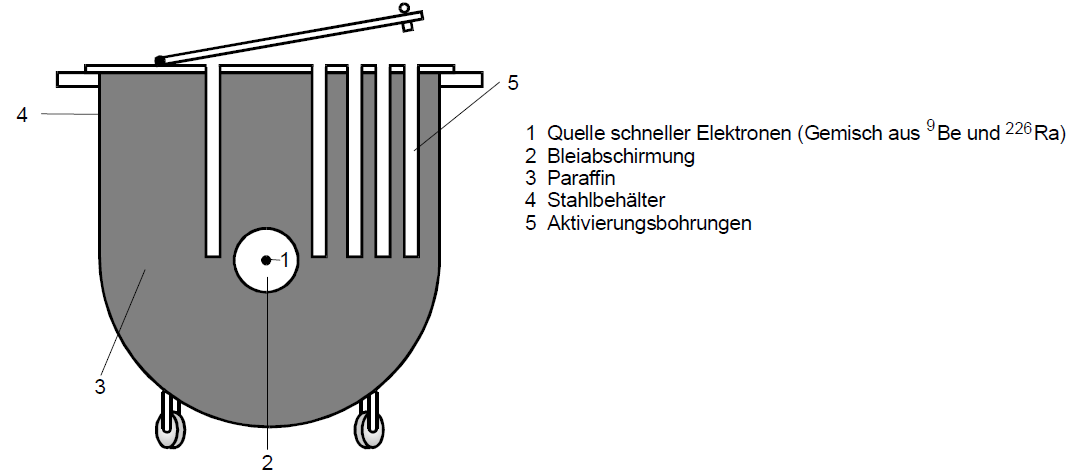
\includegraphics[width = 12cm]{img/Quelle.PNG}
			\caption{Querschnitt durch die hier verwendete Quelle f"ur thermische Neutronen}
			\label{quelle}
		\end{figure}

		Bei diesem Vorgang werden die Neutronen auf etwa $\SI{2.2}{\kilo\meter\per\second}$ abgebremst. Neutronen mit dieser Eigenschaft werden als thermische Elektronen bezeichnet.

	\subsection{Untersuchung des Zerfalls instabiler Isotope}
	\label{sub:untersuchung_des_zerfalls_instabiler_isotope}
	
		F"ur diesen Versuch wurden die Elemente $^{115}\mathrm{In}$ und $^{103}\mathrm{Rh}$ benutzt f"ur deren Zerfall gilt:

		\begin{eqnarray*}
			^{115}_{49}\mathrm{In} &+& n \rightarrow ^{116}_{49}\mathrm{In} \rightarrow ^{116}_{50}\mathrm{Sn} + \beta^- + \bar{\nu}_e,\\
			^{103}_{45}\mathrm{Rh} &+& n \left\{
			\begin{array}{ll}
			 	 \xrightarrow{10\%} & ^{104i}_{45}\mathrm{Rh} \rightarrow ^{104}_{45}\mathrm{Rh} + \gamma \rightarrow ^{104}_{46}\mathrm{Pd} +\beta^- +\bar{\nu}_e,\\
			 	  \xrightarrow{90\%} & ^{104}_{45}\mathrm{Rh} \rightarrow ^{104}_{46}\mathrm{Pd} +\beta^- +\bar{\nu}_e.
			\end{array}.
			\right.
		\end{eqnarray*}

		F"ur den Radioaktiven zerfall gilt:

		\begin{equation}
			N(t) = N_0 \exp{(-\lambda t)}. \label{zerfall}
		\end{equation}

		\begin{center}
				\tiny{($\lambda$ = Zerfallskonstante).}
		\end{center}

		Daraus folgt aus \eqref{zerfall} f"ur die Halbwertszeit aus der Zerfallskonstanten:

		\begin{eqnarray*}
			\frac{1}{2} N_0 &=& N_0 exp{(-\lambda T)},\\
			\Rightarrow \qquad T &=& \frac{\ln{2}}{\lambda}.
		\end{eqnarray*}

		Da $N(t)$ nicht zuverl"assig ermittelt werden kann, wird stattdessen $N_{\Delta t}(t)$ gemessen. 
		$N_{\Delta t}(t)$ steht dabei f"ur die in der Zeit $\Delta t$ zerfallenen Kerne.
		Dabei gilt:

		\begin{equation}
			\ln{N_{\Delta t}(t)} = \ln{N_0 (1 - \exp{-\lambda \Delta t})} - \lambda t.
		\end{equation}
		
		Daraus l"asst sich mit einer linearen Ausgleichsrechnung $\lambda$ bestimmen, da $\ln{N_0 (1 - \exp{-\lambda \Delta t})}$ konstant ist.
		So ist die Halbwertszeit von Indium zu berechnen.
		Beim Rhodium m"ussen die beiden Isotope $^{104}_{45}\mathrm{Rh}$ und $^{104i}_{45}\mathrm{Rh}$ ber"ucksichtigt werden.
		Beide besitzen unterschiedliche Halbwertszeiten und $^{104i}_{45}\mathrm{Rh}$ gibt einen zus"atzlichen $\gamma$-Quant ab, bevor es zu $^{104}_{45}\mathrm{Rh}$ wird.
		Dieser wird auch detektiert.
		$\ln{N_0 (1 - \exp{-\lambda_l \Delta t})}$ l"asst sich mithilfe einer Ausgleichsrechnung bestimmen.
		Die Formel f"ur $\lambda_k$ ergibt sich dann durch eine Ausgleichsrechnung von {$\ln$\eqref{lambdak}, $t_i$}

		\begin{eqnarray}
			N_{\Delta tl}(t) &:=& N_{0l} (1-\exp{-\lambda_l \Delta t})\exp{-\lambda_l t},\nonumber\\
			\Rightarrow \qquad N_{\Delta tk}(t_i) &=& N_{\Delta t}(t_i) - N_{\Delta tl}(t_i). \label{lambdak}
		\end{eqnarray}

		Dabei ist $t_i$ klein zu w"ahlen.